\subsubseccion{Ley multinomial}
\label{Sssec:MP:Multinomial}

Esta ley es una generalizaci\'on de la ley binomial y aparece por ejemplo cuando
se  repite  una  experiencia  a  \  $k$  \ estados  \  $n$  \  veces  de  manera
independiente y nos  interesamos a la probabilidad que  el primer evento aparece
$n_1$ veces,  el secundo  $n_2$ veces, \ldots  (ej. para  $k = 6$,  contamos los
n\'umeros de $1$, de $2$, \ldots cuando tiramos $n$ veces este dado). Apareci\'o
tambi\'en   esta   ley   por   la    primera   vez   en   el   trabajo   de   J.
Bernoulli~\cite{Ber1713, Hal90,  DavEdw01} (ver tambi\'en el  ensayo de Montmort
de 1708 con otras notaciones~\cite{Mon13}).

Se  denota  \  $X  \ \sim  \  \M(n,p)$  \  con  \  $n  \in  \Nset_0$ \  y  \  $p
= \begin{bmatrix}  p_1 & \cdots  & p_k \end{bmatrix}^t  \in \Simp{k-1}$ \  the \
$(k-1)$-simplex estandar  (ver figura~\ref{Fig:MP:Dirichlet}-(a) m\'as adelante,
y  notaciones).   Entonces,  a pesar  de  que  se  escribe  \  $X$ \  de  manera
$k$-dimensional,  el vector  partenece a  un espacio  claramente \  $d =  k-1$ \
dimensional y en el caso \ $k = 2$ \ se recupera la ley binomial.  El dominio de
definici\'on es claramente $\Part{n}{k}$ (ver notaciones). Las caracter\'isticas
de \ $X \ \sim \ \M(n,p)$ \ son las siguientes:

\begin{caracteristicas}
%
Dominio de definici\'on
%~\footnote{De hecho, se puede considerar que el vector
%aleatorio es \ $(k-1)$-dimensional \ $\widetilde{X} = \begin{bmatrix}
%\widetilde{X}_1 & \cdots & \widetilde{X}_{k-1} \end{bmatrix}^t$ \ definido sobre
%el dominio \ $\widetilde{\X} = \left\{ x \in \{ 0 \; \ldots \; n\}^{k-1}, \:
%\sum_{i=1}^{k-1} x_i \le n \right\}$.\label{Foot:MP:MultinomialDominio}}
 & $\X = \Part{n}{k}$
%\left\{ x \in \{ 0 \; \ldots \; n\}^k \tq \sum_{i=1}^k x_i = n \right\}$
\\[2mm]
\hline
%
Par\'ametros
%~\footnote{El par\'ametro de \ $\widetilde{X}$ \ es \ $\widetilde{p} =
%\protect\begin{bmatrix} p_1 & \cdots & p_{k-1} \end{bmatrix}^t\protect \in
%\left\{ q \in [0 \; 1]^{k-1} \tq \sum_{i=1}^{k-1} q_i \le 1
%\right\}$.\label{Foot:MP:MultinomialParametro}}
 & $n \in \Nset_0$, \quad $p \in
\Simp{k-1}$\\[2mm]
\hline
%
%Distribuci\'on de probabilidad
Funci\'on de masa
%~\footnote{La masa de probabilidad de \
%$\widetilde{X}$ \ es \ $p_{\widetilde{X}}(x) = \frac{n!}{\prod_{i=1}^{k-1} x_i!
%(n-\sum_{i=1}^{k-1} x_i)!}  \prod_{i=1}^{k-1} p_i^{x_i} \, \left( 1 -
%\sum_{i=1}^{k-1} p_i \right)^{n-\sum_{i=1}^{k-1}
%x_i}$.\label{Foot:MP:MultinomialMasa}}
 & $\displaystyle p_X(x) =
\frac{n!}{\prod_{i=1}^k x_i!}  \prod_{i=1}^k p_i^{x_i}$\\[2mm]
\hline
%
Promedio & $\displaystyle m_X = n p$\\[2mm]
\hline
%
Covarianza
%~\footnote{$\Sigma_X \in \Pos_k(\Rset)$, pero de \ $\uno^t \Sigma_X \uno =
%0$ \ viene \ $\Sigma_X \notin \Pos_k^+(\Rset)$. Eso es la consecuencia directa del
%hecho de que \ $X$ \ $d$-dimensional, vive sobre \ $\Simp{k-1}$,
%$(d-1)$-dimensional.\label{Foot:MP::MultinomialCovarianza}}
 & $\displaystyle
\Sigma_X = n \left( \Diag(p) - p p^t \right)$\\[2mm]
\hline
%
Generadora de probabilidad
%~\footnote{Notar: $G_{\widetilde{X}}\left(
%\widetilde{z} \right) = G_X\left( \begin{bmatrix} \widetilde{z} &
%1 \end{bmatrix}^t \right)$ \ y al rev\'es \ $G_X(z) = z_k^n \,
%G_{\widetilde{X}}\left( \begin{bmatrix} \frac{z_1}{z_k} & \cdots &
%\frac{z_{k-1}}{z_k} \end{bmatrix}^t
%\right)$.\label{Foot:MP:MultinomialGeneProba}}
 & $\displaystyle G_X(z) = \left(
p^t z \right)^n$ \ para \ $z \in \Cset^k$\\[2mm]
\hline
%
Generadora de momentos
%~\footnote{Notar: $M_{\widetilde{X}}\left( \widetilde{u}
%\right) = M_X\left( \begin{bmatrix} \widetilde{u} & 0 \end{bmatrix}^t \right)$ \
%y \ $M_X(u) = e^{n \, u_k} M_{\widetilde{X}}\left( \begin{bmatrix} u_1 - u_k &
%\cdots & u_{k-1} - u_k \end{bmatrix}^t
%\right)$.\label{Foot:MP:MultinomialGeneMomentos}}
 & \protect$\displaystyle
M_X(u) = \left( p^t e^u \right)^n, \: e^u = \begin{bmatrix} e^{u_1} & \cdots &
e^{u_k} \end{bmatrix}^t$\protect \ para \ $u \in \Cset^k$\\[2mm]
\hline
%
Funci\'on caracter\'istica
%~\footnote{Notar: $\Phi_{\widetilde{X}}\left(
%\widetilde{\omega} \right) = \Phi_X\left( \begin{bmatrix} \widetilde{\omega} &
%0 \end{bmatrix}^t \right)$ \ o \ $\Phi_X(\omega) = e^{\imath \, n \, \omega_k}
%\Phi_{\widetilde{X}}\left( \begin{bmatrix} \omega_1 - \omega_k & \cdots &
%%\omega_{k-1} - \omega_k \end{bmatrix}^t
%\right)$.\label{Foot:MP:MultinomialCaracteristica}} 
& $\displaystyle
\Phi_X(\omega) = \left( p^t e^{\imath \omega} \right)^n$
\end{caracteristicas}

% Momentos & $ \Esp\left[ X^k \right] = ??\\[2mm]
% Momento factorial & $\Esp\left[ (X)_k \right] = 
% \frac{(r+k-1)!}{(r-1)!} \left( \frac{p}{1-p} \right)^k$\\[2mm]
% Modo $\left\lfloor (n+1) p \right\rfloor$
% Mediana $\left\lfloor n p \right\rfloor$ o $\left\lceil n p \right\rceil
% CDF	$I_{1-p}(n-k,k+1)$ regularized incomplete beta function

De hecho, se puede considerar que el vector aleatorio es \ $(k-1)$-dimensional \
$\widetilde{X}     =    \begin{bmatrix}     \widetilde{X}_1    &     \cdots    &
  \widetilde{X}_{k-1}   \end{bmatrix}^t$   \  definido   sobre   el  dominio   \
$\widetilde{\X} = \left\{ x \in \{ 0 \; \ldots \; n\}^{k-1}, \: \sum_{i=1}^{k-1}
  x_i  \le n  \right\}$. El  par\'ametro de  \ $\widetilde{X}$  \ es  entonces \
$\widetilde{p}     =     \protect\begin{bmatrix}      p_1     &     \cdots     &
  p_{k-1}  \end{bmatrix}^t\protect  \in  \left\{   q  \in  [0  \;  1]^{k-1}  \tq
  \sum_{i=1}^{k-1}  q_i  \le  1  \right\}$.    La  masa  de  probabilidad  de  \
$\widetilde{X}$   \   se    escribe   obviamente   \   $p_{\widetilde{X}}(x)   =
\frac{n!}{\prod_{i=1}^{k-1} x_i!   (n-\sum_{i=1}^{k-1} x_i)!}  \prod_{i=1}^{k-1}
p_i^{x_i} \, \left( 1  - \sum_{i=1}^{k-1} p_i \right)^{n-\sum_{i=1}^{k-1} x_i}$.
Se  notar\'a al  final que  \ $G_{\widetilde{X}}\left(  \widetilde{z}  \right) =
G_X\left(  \begin{bmatrix} \widetilde{z}  & 1  \end{bmatrix}^t \right)$  \  y al
rev\'es   \   $G_X(z)  =   z_k^n   \,  G_{\widetilde{X}}\left(   \begin{bmatrix}
    \frac{z_1}{z_k}  & \cdots  &  \frac{z_{k-1}}{z_k} \end{bmatrix}^t  \right)$.
Similarmente,    \     $M_{\widetilde{X}}\left(    \widetilde{u}    \right)    =
M_X\left(  \begin{bmatrix} \widetilde{u}  &  0 \end{bmatrix}^t  \right)$  \ y  \
$M_X(u)  = e^{n  \, u_k}  M_{\widetilde{X}}\left(  \begin{bmatrix} u_1  - u_k  &
    \cdots  &  u_{k-1}  -  u_k  \end{bmatrix}^t \right)$  (y  similarmente  para
$\Phi_X$ y $\Phi_{\widetilde{X}}$).

Se puede ver  tambi\'en que $\Sigma_X \uno  = 0$ \ as\'i que  \ $\Sigma_X \notin
\Pos_k^+(\Rset)$.   Eso  es la  consecuencia  directa  del hecho  de  que  \ $X$  \
$k$-dimensional, vive sobre  \ $\Simp{k-1}$, $(k-1)$-dimensional. Aparentemente,
siendo  $\Sigma_X$  no  invertible,  no  se  puede  definir  ni  asimetr\'ia,  ni
curtosis. Sin embargo, habr\'ia que considerar \ $\widetilde{X}$, de promedio $n
\widetilde{p}$ y de covarianza el bloque $(k-1) \times (k-1)$ de $\Sigma_X$, que es
ahora invertible. $\gamma_{\widetilde{X}}$ \  y \ $\kappa_{\widetilde{X}}$ \ son
bien definidos. Las expresiones, demasiado pesadas, no son dadas ac\'a.

Deos ejemplos de masa de probabilidad de esta ley son representadas en la figura
Fig.~\ref{Fig:MP:Multinomial}.
%
\begin{figure}[h!]
\begin{center} 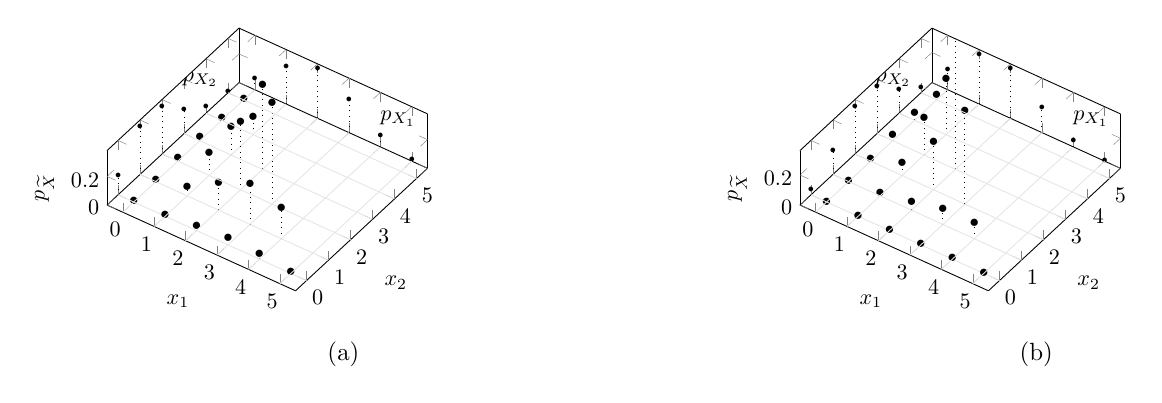
\begin{tikzpicture}[scale=.8]
\shorthandoff{>}
%
%
\pgfmathsetmacro{\n}{5};% numeros para la multinomial
\pgfmathsetmacro{\dec}{.5};% shitf para dibujar las marginales
%
% Ejemplo [6 5 4]/15
\begin{scope}
%
\pgfmathsetmacro{\pu}{2/5};% p_1
\pgfmathsetmacro{\pd}{1/3};% p_2
\pgfmathsetmacro{\qu}{floor((\n+1)*\pu)};% modo de la binomial 1
\pgfmathsetmacro{\qd}{floor((\n+1)*\pd)};% modo de la binomial 2
\pgfmathsetmacro{\mau}{factorial(\n)/factorial(\qu)/factorial(\n-\qu)*(\pu^\qu)*((1-\pu)^(\n-\qu))};% maximo de la binomial 1
\pgfmathsetmacro{\mad}{factorial(\n)/factorial(\qd)/factorial(\n-\qd)*(\pd^\qd)*((1-\pd)^(\n-\qd))};% maximo de la binomial 2
\pgfmathsetmacro{\ma}{max(\mau,\mad)};% maximo de ambas binomiales
%
\begin{axis}[
    colormap = {whiteblack}{color(0cm)  = (white);color(1cm) = (black)},
    width=.55\textwidth,
    view={35}{70},
    enlargelimits=false,
    xmin={-\dec},
    xmax={\n+\dec},
    ymin={-\dec},
    ymax={\n+\dec},
    zmax={1.1*\ma},
    color=black,
    xtick={0,...,\n},
    ytick={0,...,\n},
    xlabel=$x_1$,
    ylabel=$x_2$,
    zlabel=$p_{\widetilde{X}}$,
]
%
\pgfmathsetmacro{\bu}{(1-\pu-\pd)^\n};% coeficiente binomial por la probabilidad p1
\pgfmathsetmacro{\bd}{\bu};% coeficiente binomial por la probabilidad p2
%
\pgfmathsetmacro{\bmu}{(1-\pu)^\n};% lo mismo para la marginale 1
\pgfmathsetmacro{\bmd}{(1-\pd)^\n};% lo mismo para la marginale 2
%
\foreach \mu in {0,...,\n} {
  \foreach \md in {0,...,\n} {
    \ifnum \numexpr\mu+\md < \numexpr\n+1
      \addplot3 [dotted,domain=0:\bd,samples=2, samples y=0,color=black] (\mu,\md,\x)  node[scale=.85]{$\bullet$};
      %
      \pgfmathsetmacro{\bld}{\bd*\pd*(\n-\md)/((\md+1)*(1-\pu-\pd))};
      \global\let\bd\bld;% proba en m2 (m1 fijo) actualizado
    \fi
  }
  %
  % Marginales
  \addplot3 [dotted,domain=0:\bmu,samples=2, samples y=0,color=black] (\mu,{\n+\dec},\x)  node[scale=.55]{$\bullet$};
  \addplot3 [dotted,domain=0:\bmd,samples=2, samples y=0,color=black] ({-\dec},\mu,\x)  node[scale=.55]{$\bullet$};
  %
  % lineas (m1,m2) abajo
  \addplot3 [domain={-\dec}:{\n+\dec},samples=2, samples y=0,color=black!10] (\mu,\x,0);
  \addplot3 [domain={-\dec}:{\n+\dec},samples=2, samples y=0,color=black!10] (\x,\mu,0);
  %
  \pgfmathsetmacro{\blu}{\bu*\pu*(\n-\mu)/((\mu+1)*(1-\pu-\pd))};
  \global\let\bu\blu;\global\let\bd\blu;% proba inicial en m1 actualizada
  %
  % lo mismo para cada marginal
  \pgfmathsetmacro{\blmu}{\bmu*\pu*(\n-\mu)/((\mu+1)*(1-\pu))};
  \global\let\bmu\blmu;% proba 1 actualizada
  \pgfmathsetmacro{\blmd}{\bmd*\pd*(\n-\mu)/((\mu+1)*(1-\pd))};
  \global\let\bmd\blmd;% proba 2 actualizada
}
%
\node at (axis cs:{3*\n/4},{\n+\dec},{\mau/2})[right]{$p_{X_1}$};
\node at (axis cs:{-\dec},{3*\n/4},{\mad/2})[above]{$p_{X_2}$};
\end{axis}
\node at ({3*\n/4},-1)[scale=.9]{(a)};
\end{scope}
%
%
%
%
% Ejemplo [1 1 1]/3
\begin{scope}[xshift = 11cm]
%
\pgfmathsetmacro{\pu}{1/3};% p_1
\pgfmathsetmacro{\pd}{1/2};% p_2
\pgfmathsetmacro{\qu}{floor((\n+1)*\pu)};% modo de la binomial 1
\pgfmathsetmacro{\qd}{floor((\n+1)*\pd)};% modo de la binomial 2
\pgfmathsetmacro{\mau}{factorial(\n)/factorial(\qu)/factorial(\n-\qu)*(\pu^\qu)*((1-\pu)^(\n-\qu))};% maximo de la binomial 1
\pgfmathsetmacro{\mad}{factorial(\n)/factorial(\qd)/factorial(\n-\qd)*(\pd^\qd)*((1-\pd)^(\n-\qd))};% maximo de la binomial 2
\pgfmathsetmacro{\ma}{max(\mau,\mad)};% maximo de ambas binomiales
%
\begin{axis}[
    colormap = {whiteblack}{color(0cm)  = (white);color(1cm) = (black)},
    width=.55\textwidth,
    view={35}{70},
    enlargelimits=false,
    xmin={-\dec},
    xmax={\n+\dec},
    ymin={-\dec},
    ymax={\n+\dec},
    zmax={1.1*\ma},
    color=black,
    xtick={0,...,\n},
    ytick={0,...,\n},
    xlabel=$x_1$,
    ylabel=$x_2$,
    zlabel=$p_{\widetilde{X}}$,
]
%
\pgfmathsetmacro{\bu}{(1-\pu-\pd)^\n};% coeficiente binomial por la probabilidad p1
\pgfmathsetmacro{\bd}{\bu};% coeficiente binomial por la probabilidad p2
%
\pgfmathsetmacro{\bmu}{(1-\pu)^\n};% lo mismo para la marginale 1
\pgfmathsetmacro{\bmd}{(1-\pd)^\n};% lo mismo para la marginale 2
%
\foreach \mu in {0,...,\n} {
  \foreach \md in {0,...,\n} {
    \ifnum \numexpr\mu+\md < \numexpr\n+1
      \addplot3 [dotted,domain=0:\bd,samples=2, samples y=0,color=black] (\mu,\md,\x)  node[scale=.85]{$\bullet$};
      %
      \pgfmathsetmacro{\bld}{\bd*\pd*(\n-\md)/((\md+1)*(1-\pu-\pd))};
      \global\let\bd\bld;% proba en m2 (m1 fijo) actualizado
    \fi
  }
  %
  % Marginales
  \addplot3 [dotted,domain=0:\bmu,samples=2, samples y=0,color=black] (\mu,{\n+\dec},\x)  node[scale=.55]{$\bullet$};
  \addplot3 [dotted,domain=0:\bmd,samples=2, samples y=0,color=black] ({-\dec},\mu,\x)  node[scale=.55]{$\bullet$};
  %
  % lineas (m1,m2) abajo
  \addplot3 [domain={-\dec}:{\n+\dec},samples=2, samples y=0,color=black!10] (\mu,\x,0);
  \addplot3 [domain={-\dec}:{\n+\dec},samples=2, samples y=0,color=black!10] (\x,\mu,0);
  %
  \pgfmathsetmacro{\blu}{\bu*\pu*(\n-\mu)/((\mu+1)*(1-\pu-\pd))};
  \global\let\bu\blu;\global\let\bd\blu;% proba inicial en m1 actualizada
  %
  % lo mismo para cada marginal
  \pgfmathsetmacro{\blmu}{\bmu*\pu*(\n-\mu)/((\mu+1)*(1-\pu))};
  \global\let\bmu\blmu;% proba 1 actualizada
  \pgfmathsetmacro{\blmd}{\bmd*\pd*(\n-\mu)/((\mu+1)*(1-\pd))};
  \global\let\bmd\blmd;% proba 2 actualizada
}
%
\node at (axis cs:{3*\n/4},{\n+\dec},{\mau/2})[right]{$p_{X_1}$};
\node at (axis cs:{-\dec},{3*\n/4},{\mad/2})[above]{$p_{X_2}$};
\end{axis}
\node at ({3*\n/4},-1)[scale=.9]{(b)};
\end{scope}
%
\end{tikzpicture} \end{center}
%
\leyenda{Ilustraci\'on de una distribuci\'on  de probabilidad multinomial para \
  $k   =  3$   \   del   vector  \   $(k-1)$-dimensional   \  $\widetilde{X}   =
  \protect\begin{bmatrix}   X_1  &  X_2   \protect\end{bmatrix}^t$  \   ($X_3  =
  1-X_1-X_2$)  \ con  las marginales  \ $p_{X_1},  \: p_{X_2}$.
  %      \      (ver      notas     de      pie~\ref{Foot:MP:MultinomialDominio}
  % y~\ref{Foot:MP:MultinomialMasa}).
  Es dibujada  solamente la  distribuci\'on sobre $\widetilde{\X}$,  siendo esta
  nula afuera de  $\widetilde{\X}$.  Los par\'ametros son \  $n = 5$ \ y  \ $p =
  \protect\begin{bmatrix}      \frac25      &      \frac13     &      \frac4{15}
    \protect\end{bmatrix}^t$ (a), $p = \protect\begin{bmatrix} \frac13 & \frac12
    & \frac16 \protect\end{bmatrix}^t$ (b).}
\label{Fig:MP:Multinomial}
\end{figure}


Notar: cuando $p = \uno_i$, la variable es cierta $X = n \uno_i$.

\SZ{Otros ilustraciones para otros $n, p$?}


Vectores  de  distribuci\'on  multinomial  tienen  una  propiedade  notable  con
respecto a una permutaci\'on de variable, parecidas a la de la binomial:
%
\begin{lema}[Efecto de una permutaci\'on]\label{Lem:MP:PermutacionMultinomial}
%
  Sea \ $X \, \sim \, \M(n,p), \: p \in \Simp{k-1}$ \ y \ $\Pi \in \Perm_k$ \
  matriz \ de permutaci\'on (ver notaciones). Entonces
  %
  \[
  \Pi X \, \sim \, \M\left( n ,  \Pi p \right)
  \]
  %
\end{lema}
%
\begin{proof}
  El  resultado  es  inmediato  saliendo  de  la  funci\'on  caracter\'istica  y
  aplicando  el  teorema~\ref{Teo:MP:PropiedadesFuncionCaracteristica} (recordar
  que $\Pi^{-1} = \Pi^t$). M\'as directamente, notando la permutation \ $\sigma$
  \ tal que  \ $\Pi = \sum_{i=1}^k \uno_i \uno_{\sigma(i)}^t$, se  puede ver que \
  $\displaystyle  P(\Pi X =  x) =  P(X =  \Pi^{-1} x)  = \frac{n!}{\prod_{i=1}^k
    x_{\sigma^{-1}(i)}!}       \prod_{i=1}^k      p_i^{x_{\sigma^{-1}(i)}}     =
  \frac{n!}{\prod_{i=1}^k x_i!}  \prod_{i=1}^k p_{\sigma(i)}^{x_i}$ \ por cambio
  de indices.
\end{proof}
%
Adem\'as, la ley multinomial  exhibe una stabilidad reemplazando dos componentes
por su suma:
%
\begin{lema}[Stabilidad por agregaci\'on]\label{Lem:MP:StabAgregacionMultinomial}
%
  Sea  \ $X =  \begin{bmatrix} X_1  & \cdots  & X_k  \end{bmatrix}^t \,  \sim \,
  \M(n,p), \:  p \in \Simp{k-1}$ \ y  \ $G^{(i,j)}$ \ matriz  de agrupaci\'on de
  las $(i,j)$-\'esima componentes (ver notaciones). Entonces,
  %
  \[
  G^{(i,j)} X \, \sim \, \M\left( n , G^{(i,j)} p \right)  
  \]
  %
\end{lema}
%
Este resultado es intuitivo del hecho que vuelve a agrupar los estados \ $i$ \ e
\ $j$  \ en un  estado, que tiene  entonces la probabilidad \  $p_i + p_j$  \ de
aparecer.
%
\begin{proof}
  Suponemos $i <  j$ (el otro caso  se recupera por simetr\'ia). A  partir de la
  funci\'on                 caracter\'istica                 y                el
  teorema~\ref{Teo:MP:PropiedadesFuncionCaracteristica} se tiene,
  %
  \begin{eqnarray*}
  \forall \: \omega \in \Rset^{k-1}, \quad \Phi_{G^{(i,j)} X}(\omega) & = &
  \Phi_X\left( G^{(i,j) \, t} \omega \right)\\[2mm]
  %
  & = & \left( \sum_{l=1}^k p_l \, e^{\imath \, \left( G^{(i,j) \, t} \omega \right)_l } \right)^n
  \end{eqnarray*}
  %
  Ahora,  se nota  que \  $G^{(i,j) \,  t} \omega  = \begin{bmatrix}  \omega_1 &
    \cdots    &   \omega_{j-1}   &    \omega_i   &    \omega_{j+1}   &    \cdots   &
    \omega_{k-1} \end{bmatrix}^t$, entonces
  %
  \begin{eqnarray*}
  \forall \: \omega \in \Rset^{k-1}, \quad \Phi_{G^{(i,j)} X}(\omega) & = &
  \left( \sum_{l=1, l \ne j}^k p_l \, e^{\imath \, \omega_l} + p_j \, e^{\imath \,
  \omega_i } \right)^n\\[2mm]
  %
  & = & \left( \sum_{l=1, l \ne i, l \ne j}^k p_l \, e^{\imath \, \omega_l} +
  (p_i+p_j) \, e^{\imath \, \omega_i } \right)^n
  %
  \end{eqnarray*}
  %
  lo que  cierra la  prueba. Se puede  tener un  enfoque m\'as directo,  con los
  mismos         pasos        que         en        la         prueba        del
  lema~\ref{Lem:MP:StabAgregacionHipergeomMulti}    tratando     de    la    ley
  hipergeometrica multivaluada.
\end{proof}

De este lema, aplicado de manera recursiva, se obtiene los corolarios siguientes:
%
\begin{corolario}\label{Cor:MP:MarginalMultinomial}
%
  Sea  \ $X  \,  \sim \,  \M(n,p)$, entonces  \  $\displaystyle X_i  \, \sim  \,
  \B(n,p_i)$.
\end{corolario}


Al  final,  por  una  an\'alisis  combinatorial,  se  muestra  sencillamente  un
resultado similar al de la binomial como suma de Bernoulli independientes:
%
\begin{lema}\label{Lem:MultinomialSumaMultiBernoulli}
%
  Sean \ $U_i, \quad i  = 1, \ldots , n$ \ discretas sobre $\U  = \{ 1 \; \ldots
  \;  k   \}$  de  masa  de   probabilidad  $p_{U_i}  =   p  \in  \Delta_{k-1}$,
  independientes, y $X_i  = \uno_{U_i}$ vectores aleatorios $k$-dimensionales
  (son, por construcci\'on, independientes). Entonces
  %
  \[
  \sum_{i=1}^n X_i \, \sim \, \M(n,p)
  \]
\end{lema}

\

Nota: esta ley  se generaliza de la misma manera que  para la binomial negativa,
dando una  ley multinomial negativa  o, de manera equivalente,  generalizando la
binomial  negativa  a  m\'as  de  dos  clases  se  obtiene  la  ley  multinomial
negativa. \SZ{Anadirlo en una seccion?}
